\chapter{Resourcefulness, Leverage, and Scale on the Las Vegas Strip}

This School of Hard Knocks chapter, prepared through Video2Book and curated by LazyingArt LLC, is built from a field interview rather than a blackboard lecture. Even so, it has a recognizable mathematical skeleton. The host first turns Las Vegas into a quantified money field, then samples a sequence of entrepreneurs, and in each case moves from visible output to hidden mechanism. Our task is to keep that motion intact. We preserve the transcript's numbers exactly where they are concrete, and where the speakers move from arithmetic to causation we translate their claims into cautious bookkeeping identities, update rules, and simple decision diagrams.

\section{Las Vegas as a Money Field}

The lecture begins with a teaser reel: annual figures, millionaire ages, and quick declarations of commercial identity. We should not read that montage as one continuous conversation. It is a compressed announcement that the city contains several different wealth mechanisms. The first real stabilizing move is numerical:
\begin{equation}
S_{\mathrm{LV}} = 45\times 10^9\,\mathrm{USD}.
\end{equation}
This is the stated amount of money spent in Las Vegas over the past year. Once that scalar is placed on the table, the city becomes more than a glamorous backdrop. It becomes an environment dense with commercial flows, and the interviews become local probes into that larger field.

\begin{table}[h]
\centering
\begin{tabular}{|l|l|l|l|l|}
\hline
Case & Vehicle & Years stated & Largest stated figure & Milestone \\
\hline
First Lamborghini & Trading + entrepreneurship & 4 & \$1.5 million & first million at 21 \\
Manufacturing & Medical supplies / paint & not stated & \$5.4 million & age 45 \\
Real estate & Real estate & 20 & tens of millions & long-run asset builder \\
Airbnb & Airbnb & 3 & nearly \$7 million & first million at 20 \\
\hline
\end{tabular}
\caption{Transcript-backed numerical anchors for the main cases.}
\end{table}

Already the host's method is clear. He begins with comparability: what do you do, how long have you done it, what was your biggest year, how old are you, when did the first million arrive? These are not idle status questions. They certify that the speaker can be treated as evidence before the lecture asks for principle.

\section{Early Wealth, Delegation, and Earned Scarcity}

The first long case concerns a young entrepreneur in a Lamborghini. The credentials are sharp: he trades full time, has been a business owner for about four years, had a best year of \$1.5 million, and made his first million at twenty-one. The obvious temptation is to collapse the whole episode into one sentence: a young trader got rich in a favorable market. The lecture itself resists that flattening.

When the host asks how the first million happened, the first answer is indeed historical timing: trading during a period when, in the speaker's own telling, money was unusually easy to make. But he immediately corrects that explanation. He says he was not really at seven figures until he delegated. That is the first major conceptual turn. Timing may open the door, but scale requires a structure larger than the founder.

We can formalize the point in the minimal way the transcript supports. Let \(Y_{\mathrm{self}}\) be what the founder can produce alone, and let \(Y_i\) be the contribution of each delegated person or component. Then
\begin{align}
Y_{\mathrm{solo}} &= Y_{\mathrm{self}},\\
Y_{\mathrm{team}} &= Y_{\mathrm{self}} + \sum_{i=1}^{n} Y_i.
\end{align}
This is not a spoken formula; it is a faithful compression of the interview's claim. Seven-figure scale appears when the business ceases to be identical with one person's hands and hours.

The lecture does not treat delegation as mechanical outsourcing. The speaker gives conditions for durable delegation: treat people well, pay them well, and create room for growth. So the equation above is not merely additive labor. It encodes an organizational claim: productive capacity rises only if the delegated pieces remain stable enough to keep contributing.

\subsection{Question \& Answer}

\paragraph{Question.} If the first million partly came during an unusually easy market, what turns that temporary opportunity into durable wealth?

\paragraph{Answer.} The lecture's answer is that timing is not sufficient. A favorable market can generate gains, but durable wealth begins only when the founder creates a structure that can carry more than founder-only output. In transcript language, that means delegation, team-building, and incentives that keep the team intact. The windfall may begin the story, but organization determines whether the story continues.

The interview then shifts from mechanism to formation. The host asks whether the speaker has ever been broke. This is one of the lecture's recurring pressure tests, and it matters because it reveals whether present scale came from inheritance, accident, or pressure. The speaker says he was raised by a single mother who never gave him anything and made him earn what he had. That answer reinterprets the earlier success. The decisive input is not luxury, but earned scarcity. One might say that the commercial system was already being trained long before the business existed.

\section{Focus, Faith, and Action Before Readiness}

The first case does not end with delegation. It moves through three deeper layers: focus, faith, and tempo.

First comes focus. The speaker says that many successful people he sees are married, and he treats marriage as a focusing device. The point is not sentimental. It is operational: remove enough external fragmentation, and effort begins to compound rather than scatter.

Next comes faith. The speaker says that God must be at the center of everything and then describes asking for a seven-figure business but receiving lessons rather than immediate reward. Teams split, business becomes shaky, and only after that does he say that things became rock solid again. The theological content belongs to the transcript and should remain there. What we can formalize is its business meaning: disorder is interpreted not as a terminal failure, but as a sequence of corrective lessons.

\paragraph{Remark.} The transcript associates ``Ephesians 3.20'' with language that appears to come from elsewhere. We therefore keep the operational claim of the passage but do not treat the citation as textually secure.

Finally, the lecture arrives at the most portable operational rule in the first case: do not wait for total completeness. Begin, expose the defects, repair them, and move again. A compact reconstruction is
\begin{equation}
Q_{t+1} = Q_t + \phi\,\Delta_t,
\qquad
\Delta_t = h(A_t),
\end{equation}
where \(A_t\) is the action taken at stage \(t\), \(\Delta_t\) is the defect set exposed by that action, and \(Q_t\) is the business quality or operating robustness at that stage. The transcript never writes such a formula, but it clearly narrates this logic.

\begin{figure}[h]
\centering
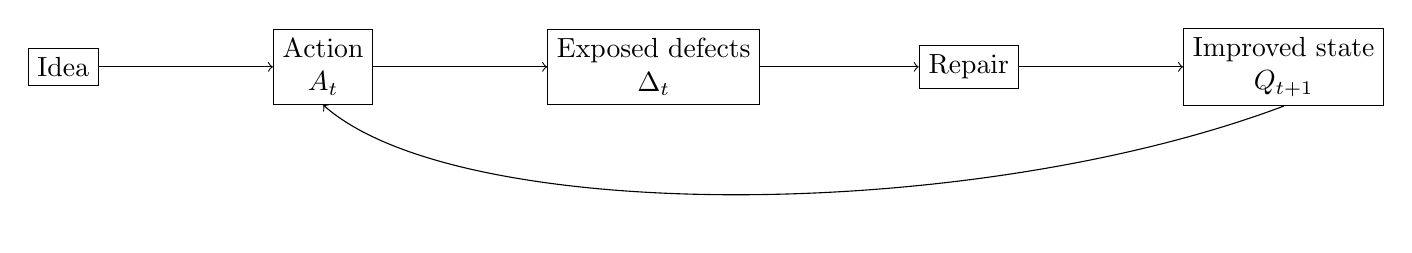
\begin{tikzpicture}[x=1cm,y=1cm]
\node[draw, align=center] (idea) at (0,0) {Idea};
\node[draw, align=center] (act) at (3.3,0) {Action\\$A_t$};
\node[draw, align=center] (gap) at (7.5,0) {Exposed defects\\$\Delta_t$};
\node[draw, align=center] (repair) at (11.5,0) {Repair};
\node[draw, align=center] (quality) at (15.5,0) {Improved state\\$Q_{t+1}$};

\draw[->] (idea) -- (act);
\draw[->] (act) -- (gap);
\draw[->] (gap) -- (repair);
\draw[->] (repair) -- (quality);
\draw[->] (quality.south) .. controls (11.5,-2) and (5,-2) .. (act.south);
\end{tikzpicture}
\caption{Transcript-derived action loop: action reveals what planning alone cannot, and repair raises the next operating state.}
\end{figure}

\subsection{Question \& Answer}

\paragraph{Question.} Why should we act before the plan is complete?

\paragraph{Answer.} Because incompleteness is not removed by waiting. It is removed by reality-testing. Action generates information that pure planning cannot generate. Once defects are visible, they become repairable. That is why the speaker dismisses the fantasy of a finished plan and urges immediate execution instead.

The host's recap after this interview compresses the case toward faith, and that compression is part of the lecture's rhythm. But we should not let the recap erase the earlier mechanism. The full movement of the case is stronger: market opportunity, delegation, earned scarcity, focus, faith, and then iterative action.

\section{Legacy, Seller Identity, and the Long Game}

The second long case shifts from youthful speed to middle-aged scale. The interviewee works in manufacturing, specifically medical supplies and military-grade paint, and reports \$5.4 million in his best year. He is forty-five. Here the lecture is no longer asking how someone moved fast; it is asking what horizon commercial life should have.

The key statement is a proverb: the world becomes a better place when a man plants seeds for future generations whose shade he will never enjoy. The host immediately asks him to unpack it. The answer is that one does not hustle merely for oneself. One hustles for family, for lineage, for the name that continues beyond the present self.

\begin{table}[h]
\centering
\begin{tabular}{|l|l|l|}
\hline
Horizon & Object of effort & Economic meaning \\
\hline
Immediate self & Personal consumption & short payoff, narrow objective \\
Family name & Household and descendants & delayed payoff, durable motive \\
Future generations & Children and grandchildren & legacy as a long-run project \\
\hline
\end{tabular}
\caption{Transcript-derived long-game matrix from the manufacturing interview.}
\end{table}

This changes the effective objective function. If the horizon is merely personal enjoyment, action can become short and brittle. If the horizon is generational, then present sacrifice can be rational even when the full benefit is deferred. The lecture makes this vivid by shifting from the first name to the last name: not merely James, but Dumoulin; not merely the front of the jersey, but the name on the back.

The same interview then reconnects to an earlier motif. The speaker says he is a seller by nature, and that seller identity is part of why he became an entrepreneur. This is not presented as technique. It is presented as disposition.

\subsection{Question \& Answer}

\paragraph{Question.} Which matters more, mindset or skill set?

\paragraph{Answer.} The interview answers: mindset. The reason given is portability. A fixed skill set can become local and rigid. A growth-oriented mindset crosses contexts. The same person can enter the mail room and refuse to remain permanently identified with it. The point is not that skill is unimportant. It is that skill without expansive orientation becomes static, while mindset keeps reopening the space of possible skills.

This case closes, once again, with faith, now named less as foundation and more as moral compass and ego restraint. That recurring movement is one of the lecture's signatures: commercial ambition is allowed, but it is repeatedly placed under something higher.

\section{Resourcefulness, Assets, and the Affordability Trap}

The real-estate interview is the lecture's analytic center. The speaker says he has been in real estate for almost twenty years and has made tens of millions in revenue and net profit. Once again, scale is the credential, not the endpoint. The interview immediately turns to origin.

The decisive shift is the distinction between money and resources. The speaker says he did not come from money, but he did come from resources, and then widens the claim: we all come from resources. What is scarce is not always the resources themselves, but the willingness to recognize them and activate them. In a compact notation,
\begin{equation}
Z_{\mathrm{usable}} = u\,Z_{\mathrm{available}},
\qquad
u\in\{0,1\}.
\end{equation}
Here \(Z_{\mathrm{available}}\) is the stock of accessible helpers, openings, and opportunities, and \(u\) is the decision to activate them by asking. If \(u=0\), the resource stock remains present but economically inert.

\subsection{Question \& Answer}

\paragraph{Question.} Do we lack resources, or do we lack resourcefulness?

\paragraph{Answer.} The lecture's answer is that the latter is often the true bottleneck. The speaker says that people willing to help him did exist, but that help became real only when he had the nerve and humility to ask. Lack of money, then, is not identical with lack of reachable assistance. The decisive variable may be whether one turns available help into usable help.

The interview then makes an even sharper turn. The speaker says that one cannot save one's way to being rich. The host recognizes at once that this is a major replacement of framework, not a motivational slogan. The criticized logic is static:
\begin{equation}
P \le I-E,
\end{equation}
where \(P\) is the price of the desired object, \(I\) is current income, and \(E\) is the current expense burden. On this view one asks only whether the object fits inside the current budget.

The speaker replaces that logic with a growth logic:
\begin{align}
I_{\mathrm{total}} &= I_{\mathrm{labor}} + C_{\mathrm{assets}},\\
C_{\mathrm{monthly}} &= N\,\bar c,\\
R_{\mathrm{annual}} &\approx 12\,C_{\mathrm{monthly}}.
\end{align}
This is the cleanest mathematical compression of his claim. Wealth does not chiefly come from shrinking the left-hand side of the household ledger. It comes from enlarging the right-hand side through cash-flowing assets. In his own preferred example, those assets are rental properties.

\begin{table}[h]
\centering
\begin{tabular}{|l|l|l|}
\hline
Question & Object examined & Likely conclusion \\
\hline
Can I afford it now? & current income minus expenses & static ceiling \\
How do I make it pay me? & labor income plus asset cash flow & expandable system \\
\hline
\end{tabular}
\caption{The transcript's contrast between the affordability question and the asset-building question.}
\end{table}

\begin{figure}[h]
\centering
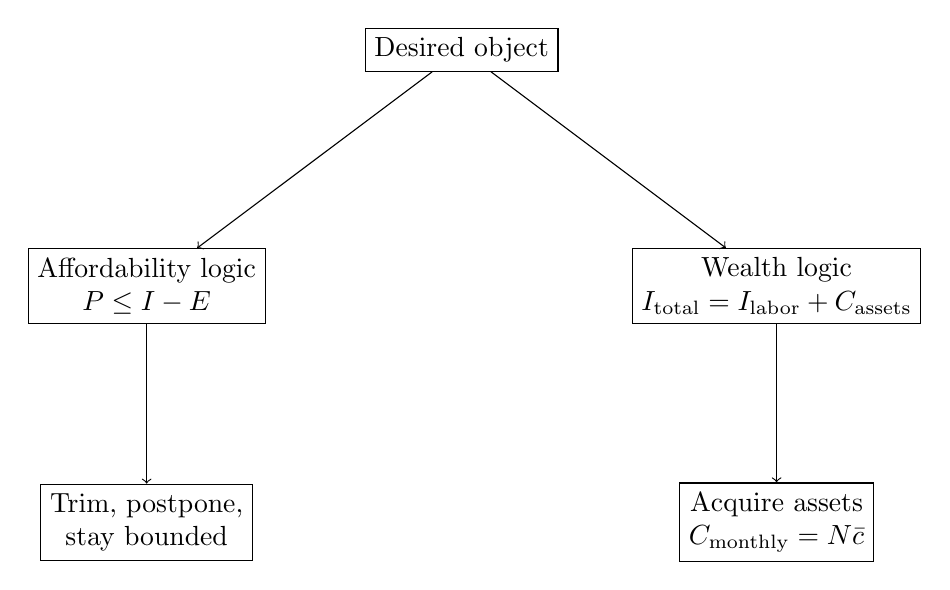
\begin{tikzpicture}[x=1cm,y=1cm]
\node[draw, align=center] (start) at (0,0) {Desired object};
\node[draw, align=center] (left) at (-4,-3) {Affordability logic\\$P \le I-E$};
\node[draw, align=center] (left2) at (-4,-6) {Trim, postpone,\\stay bounded};
\node[draw, align=center] (right) at (4,-3) {Wealth logic\\$I_{\mathrm{total}} = I_{\mathrm{labor}} + C_{\mathrm{assets}}$};
\node[draw, align=center] (right2) at (4,-6) {Acquire assets\\$C_{\mathrm{monthly}} = N\bar c$};

\draw[->] (start) -- (left);
\draw[->] (start) -- (right);
\draw[->] (left) -- (left2);
\draw[->] (right) -- (right2);
\end{tikzpicture}
\caption{Transcript-derived bifurcation: static affordability versus expandable cash flow.}
\end{figure}

\subsection{Question \& Answer}

\paragraph{Question.} Why, in this lecture's logic, can we not save our way to wealth?

\paragraph{Answer.} Because saving by itself operates on a bounded flow. It can reduce waste and extend runway, but it does not by itself create the expanding side of the ledger. The speaker's argument is not anti-discipline; it is anti-static thinking. If the question remains only whether today's income can absorb today's purchase, then the scale of life is bounded by present labor. Wealth begins when income-producing assets enter the system.

The lecture then broadens into a diagnosis of distraction. Politics, football, alcohol, and more general numbing routines are described as drains on ambition. This is rhetorical rather than measured, and we should preserve that status. Still, the interview is making a clean contrast between two states:

\begin{table}[h]
\centering
\begin{tabular}{|l|l|l|}
\hline
State & Dominant condition & Claimed outcome \\
\hline
Distracted state & numbing routines, low focus & ambition washed away \\
Undistracted state & necessity, concentration & constructive agency reappears \\
\hline
\end{tabular}
\caption{Transcript-derived contrast between distracted and undistracted modes of action.}
\end{table}

The wilderness example is the speaker's metaphor for this second state. Remove distraction, and the person begins to build shelter, find water, and devise survival methods. We do not turn this into a measured production function. We simply note the claim: under concentration and necessity, the human being becomes a maker again.

The interview closes on sacrifice. Health, family, friend groups, sanity: these are listed as costs. That matters. The asset logic of the section should not be misread as frictionless compounding. The lecture insists that scale has a price.

\section{From Time-for-Money to Scalable Units}

The final major case returns to Airbnb, but now in operational rather than teaser form. The speaker says she used to nanny, that COVID interrupted the job structure, and that the deeper problem was not only instability but ceiling. A job organized as time-for-money can be respectable and still feel structurally limited:
\begin{equation}
R_{\max}^{\mathrm{wage}} = w\,h_{\max}.
\end{equation}
Here \(w\) is the effective hourly rate and \(h_{\max}\) is the maximum labor time available. However hard one works, the form itself imposes a bound.

That is why the interview turns toward leverage. The speaker says she did not want other people dictating whether she would have income, and she did not want every additional dollar to require one more hour. She then says that business credit became visible to her as a lever. The transcript gives no interest rates, limits, or repayment structure, so we do not write a debt model. We keep the narrower and safer point: seed capacity, whether from job income or credit, can be used to create units that generate income without identical increments of labor.

\subsection{Question \& Answer}

\paragraph{Question.} What can someone at rock bottom do right now?

\paragraph{Answer.} The lecture gives a practical two-part answer. First, if there is already a job, treat that cash flow as seed capacity rather than pure consumption. Second, if business credit is accessible, use it to acquire or control an income-producing unit rather than a consumption good. The emphasis is not elegance but movement. One begins with the first tractable paying unit.

The Airbnb case gives enough numbers for a small worked example. The speaker reports an early level of about \$3{,}000 per month, then about \$60{,}000 per month, and then nearly \$400{,}000 in the first calendar year:
\begin{align}
M_0 &\approx \$3{,}000/\text{month},\\
M_1 &\approx \$60{,}000/\text{month},\\
R_{\text{year 1}} &\approx \$400{,}000.
\end{align}
Here \(M_0\) and \(M_1\) should be read as monthly business levels as described in the interview; the transcript does not supply a finer accounting distinction. We can now check the internal arithmetic.

\paragraph{Worked derivation.}
\begin{enumerate}
\item If the first calendar year produced approximately \$400{,}000, then the average monthly level over that year was
\begin{equation}
\bar M_{\text{year 1}} = \frac{R_{\text{year 1}}}{12} \approx \frac{\$400{,}000}{12} \approx \$33{,}333/\text{month}.
\end{equation}
\item If the later run rate of \$60{,}000 per month had held for the entire year, then the annual total would have been
\begin{equation}
12\times \$60{,}000 = \$720{,}000.
\end{equation}
\item Since \$720{,}000 is well above the reported \$400{,}000, the \$60{,}000 level cannot have been present throughout the entire first year.
\item Therefore the run rate must have ramped during the year rather than staying flat from the start.
\end{enumerate}

This small calculation matters because it protects the lecture from sounding magical. The speaker herself says it is a numbers game. The arithmetic agrees: scale arrived by ramp, not by immediate steady state.

Once that is in place, the final operational rule is simple. Airbnb was not presented as metaphysically special; it was the first vehicle that worked. If a person can buy, then buy. If not, rent and control the first unit. Then scale the count \(N\) of functioning units, provided the properties are winners and the average per-unit cash flow remains positive:
\begin{equation}
C_{\mathrm{monthly}} = N\,\bar c.
\end{equation}
At this point the lecture has reached its cleanest practical form. The business becomes a countable system of units rather than an unbounded cloud of motivation.

\section{Summary}

The lecture begins with spectacle and ends with structure. First we are given a city-level scalar, \(S_{\mathrm{LV}}\), and the promise that Las Vegas can be read as a dense field of commercial evidence. Then the host moves from case to case in a stable rhythm: credential, origin, principle, recap, next test. A young trader teaches that market opportunity must be converted into organization. A manufacturer turns ambition from self-consumption toward legacy and lineage. A real-estate operator replaces the affordability question with the asset question and insists that the crucial scarcity is often resourcefulness rather than resources. An Airbnb entrepreneur closes by turning the rejection of wage ceilings into a scale path measured in units and run rates.

What remains, once we remove the glamour and the compression of the recaps, is a coherent sequence of mechanisms. We move from founder-bound output to team output, from planning to action-feedback, from static affordability to cash-flow assets, and from time-for-money exchange to scalable units. No validated board equations survive from the visual record, but the transcript itself supplies enough numerical and causal structure to let the lecture unfold as a serious set of notes.